\section{Integration Strategy}

\subsection{Entry Criteria}
\label{sec:entryCriteria}
The following conditions have to be verified before entering the integration testing phase in order for it to produce meaningful results.\\

A fundamental initial criterion is that the development of the components and their functionalities proceeds together with the unit testing on such components, so that even when the components are not fully developed, they have already been tested at unit level w.r.t. the fully developed functionalities. 
Given the aforementioned criterion, before entering the integration phase, the development percentage of a component must be at least 90\% and the main functionalities required to test its integration w.r.t. another component of the system must be fully developed.\\

The integration process can start when these conditions are met by the system development
\begin{itemize}
	\item 100\% of development on the \emph{Data Provider} component
	\item 90\% of development on the \emph{Event Broker} and \emph{Car Handler} components
	\item 80\% of development on the \emph{Rent Manager} component
	\item 60\% of development on the \emph{Maintenance Manager} component
	\item 40\% of development on the \emph{User Information Manager} and \emph{Access Manager} components
	\item 30\% of development on the \emph{User Application Server}, \emph{User Application}, \emph{Customer Care Server} and \emph{Customer Care Application} components
\end{itemize}

\subsection{Elements to be integrated}
In this section we identify the components and subcomponents to be integrated and add some details about their specific integration.\\

As specified in the design document, some component of the PowerEnJoy system such as the \emph{Rent Manager} and the \emph{Maintenance Manager} are rather complex and thus its internal subcomponents need to be integrated before proceeding with the integration of entire components with other components of the system.\\

The following components will be integrated to obtain the subsystem related to the Maintenance functionalities:

\begin{itemize}
	\item \emph{Maintenance Manager}
	\item \emph{Event Broker}
	\item \emph{Data Provider}
	\item \emph{Car Handler}
\end{itemize}

The following components will be integrated to obtain the subsystem related to the User Application functionalities:

\begin{itemize}
	\item \emph{User Application}
	\item \emph{UserApp Server}
	\item \emph{Access Manager}
	\item \emph{Rent Manager}
	\item \emph{User Information Manager}
	\item \emph{Data Provider}
	\item \emph{Car Handler}
	\item \emph{Event Broker}
\end{itemize}

The following components will be integrated to obtain the subsystem related to the Customer Care functionalities:

\begin{itemize}
	\item \emph{Customer Care Application}
	\item \emph{Customer Care Server}
	\item \emph{User Information Manager}
	\item \emph{Data Provider}
\end{itemize}

\paragraph{Notes}
The external components like the \emph{DBMS} and the external APIs are products that are not developed by us and that we suppose already completely tested; however we decided to include them in the integration testing by firstly testing the external component's interfaces on their own, and the by proceeding to test them when integrated with PowerEnJoy components.\\
In the same way the Maintenance Manger will be tested as a component integrated with our system and then it will be tested through the Maintenance API it provides to the maintenance company. 

\subsection{Integration Testing Strategy}
Both bottom-up and top-down were taken in consideration when thinking of the integration strategy for the PowerEnJoy system; looking at the structure and composition of the system it is clear the most complex and relevant functionalities are located in the lower end tiers, which are also the most independent ones. Moreover as stated in \hyperref[sec:entryCriteria]{Section 2.1} those will be the only fully developed components at the time of starting the integration process since the software development of the PowerEnJoy system will proceed using the bottom-up approach. These considerations brought us to lean towards a bottom-up approach that will allow the lower end components to be tested and integrated before any other component; doing so any issue or problem in the integration phase of these components will be found at an early stage in the integration process, and so it will be easier to tackle it and solve it, while maintaining as much parallelism and decoupling as possible.\\
Given that some functionalities of the system are decoupled, during the integration process some steps of the integration sequence will have the same priority. In those cases the critical-module-first approach will be used in order to integrate and test the riskiest  components first and solve their issues before they create worse problems in the integration process.
\subsection{Sequence of Component Integration}
Depends on strategy chosen, this is a proposed structure.

\subsubsection{Overall Component Integration Diagram} 
The diagram above shows the needed precedences in the integration phase between the main components of the system.

	\begin{figure}[h]
			\centering
			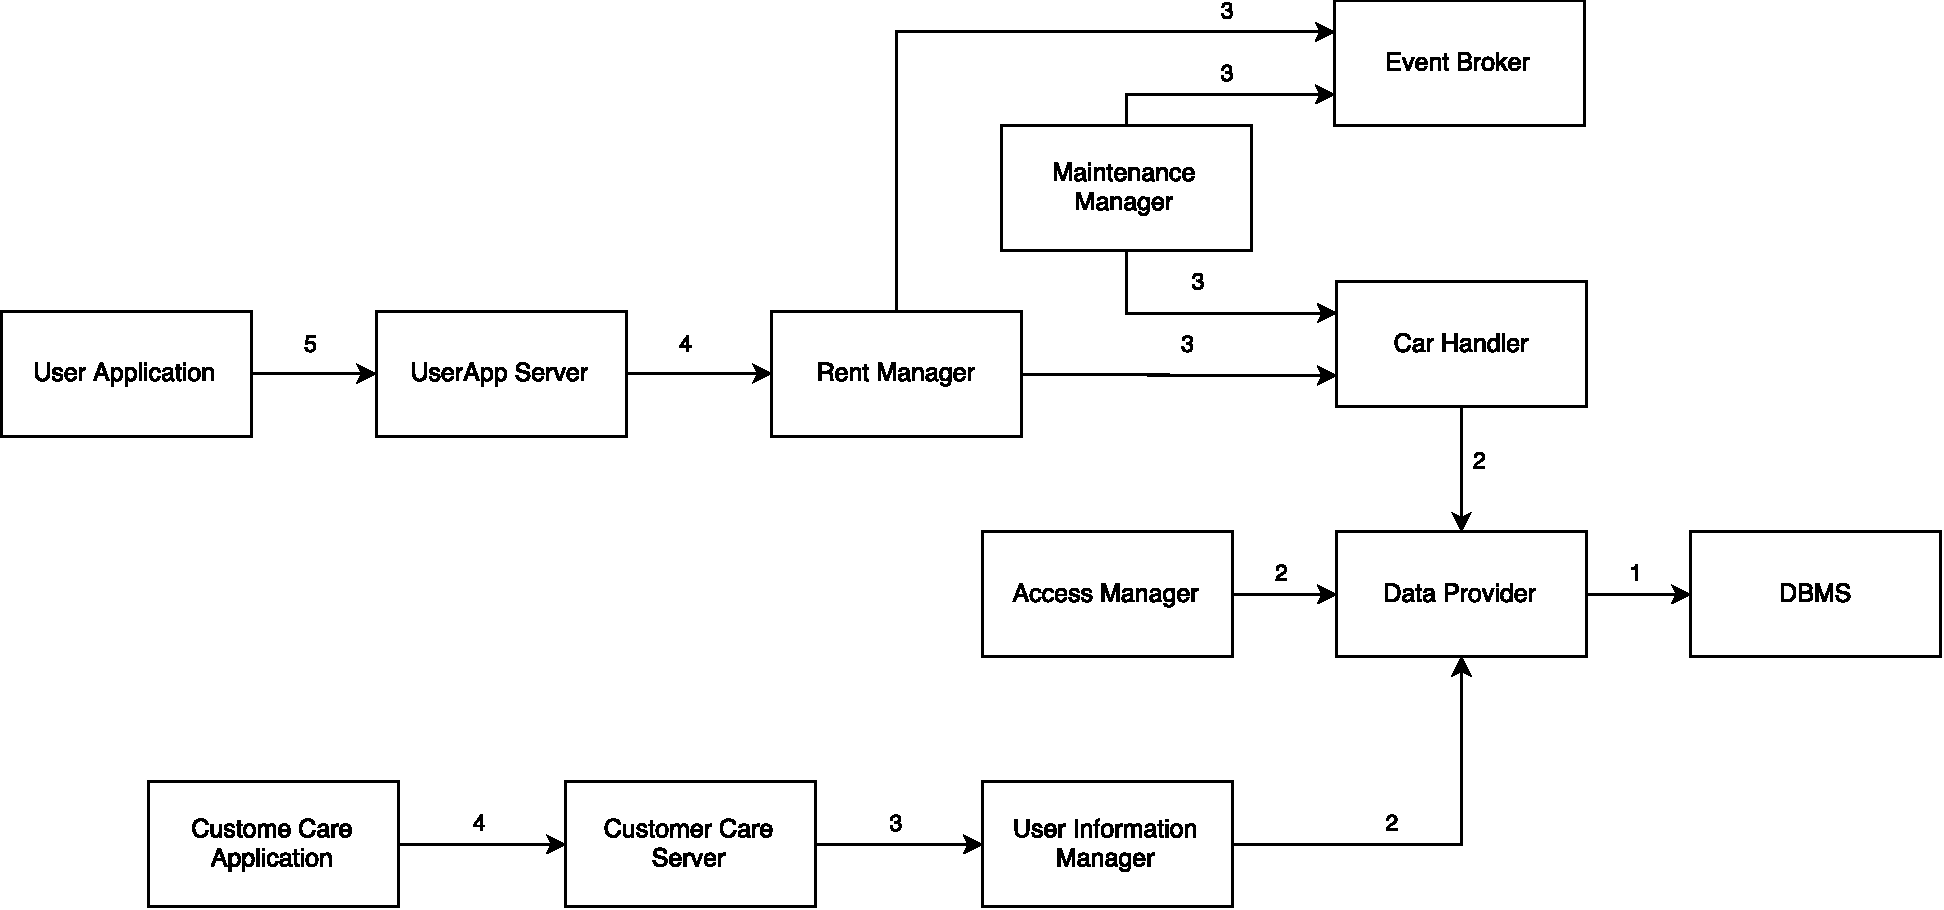
\includegraphics[width=\linewidth]{img/overallIntegration}
			\caption{
				\label{fig:overallIntegration} 
				\emph{Overall Component Integration Diagram}
			}
	\end{figure}

\clearpage

\subsubsection{Subcomponent Integration} 
Fare unit test con attenzione a queste precedenze nei seguenti componenti.
\todo{tradurre e sistemare}

\paragraph{RentManager} 
The diagram above shows the needed precedences in the integration phase inside the \emph{RentManager} component.
\paragraph{}

		\begin{figure}[h]
			\centering
			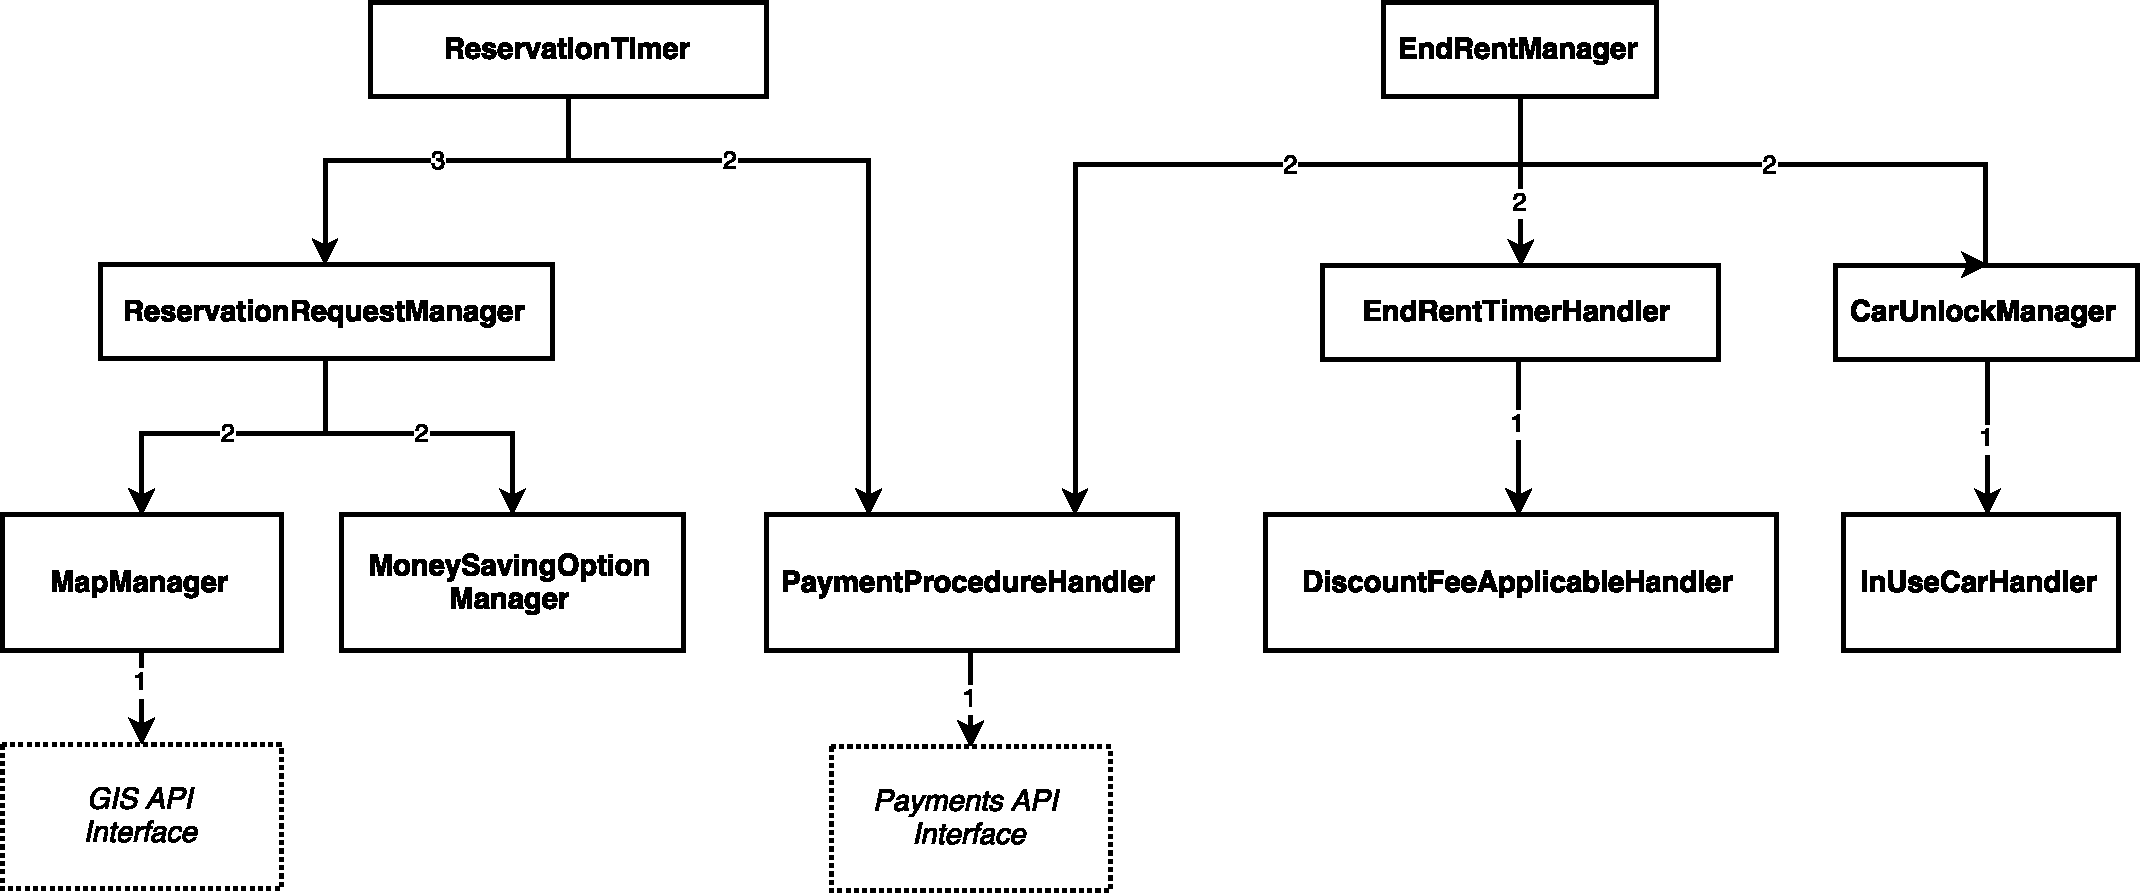
\includegraphics[width=\linewidth]{img/rentManagerIntegration}
			\caption{
				\label{fig:rentManagerIntegration} 
				\emph{RentManager integration}
			}
		\end{figure}
		
\paragraph{MaintenanceManager} 
The diagram above shows the needed precedences in the integration phase inside the \emph{MaintenanceManager} component.
\paragraph{}

		\begin{figure}[h]
			\centering
			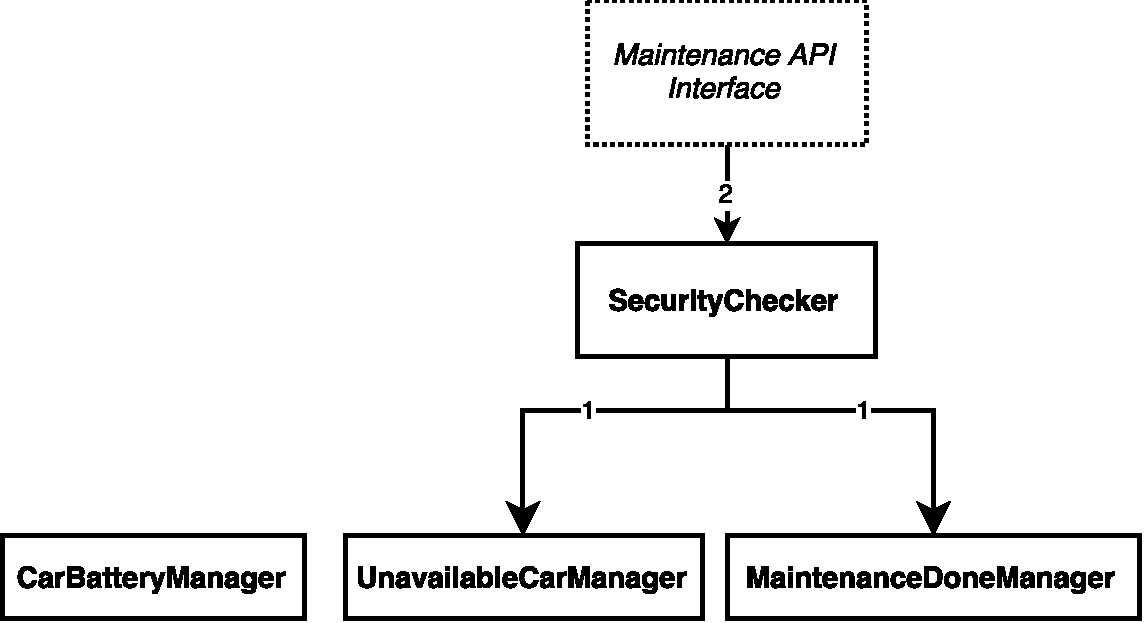
\includegraphics[width=\linewidth]{img/maintenanceIntegration}
			\caption{
				\label{fig:maintenanceIntegration} 
				\emph{MaintenanceManager integration}
			}
		\end{figure}
		
\paragraph{UserInformationManager} 
The diagram above shows the needed precedences in the integration phase inside the \emph{UserInformationManager} component.
\paragraph{}

		\begin{figure}[h]
			\centering
			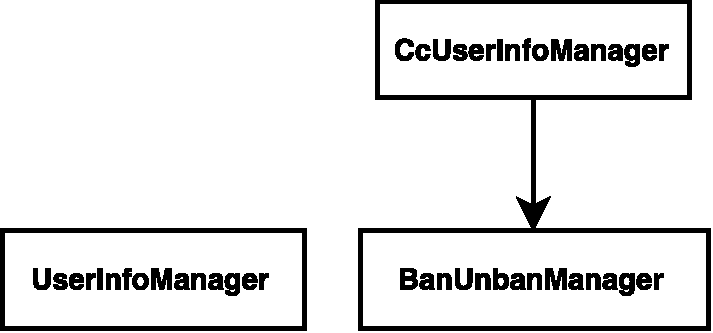
\includegraphics[width=0.6\linewidth]{img/userIntegration}
			\caption{
				\label{fig:userIntegration} 
				\emph{UserInformationManager integration}
			}
		\end{figure}

\clearpage

\subsubsection{Component Integration}

\paragraph{DataProvider} 
...
\paragraph{}

		\begin{figure}[h]
			\centering
			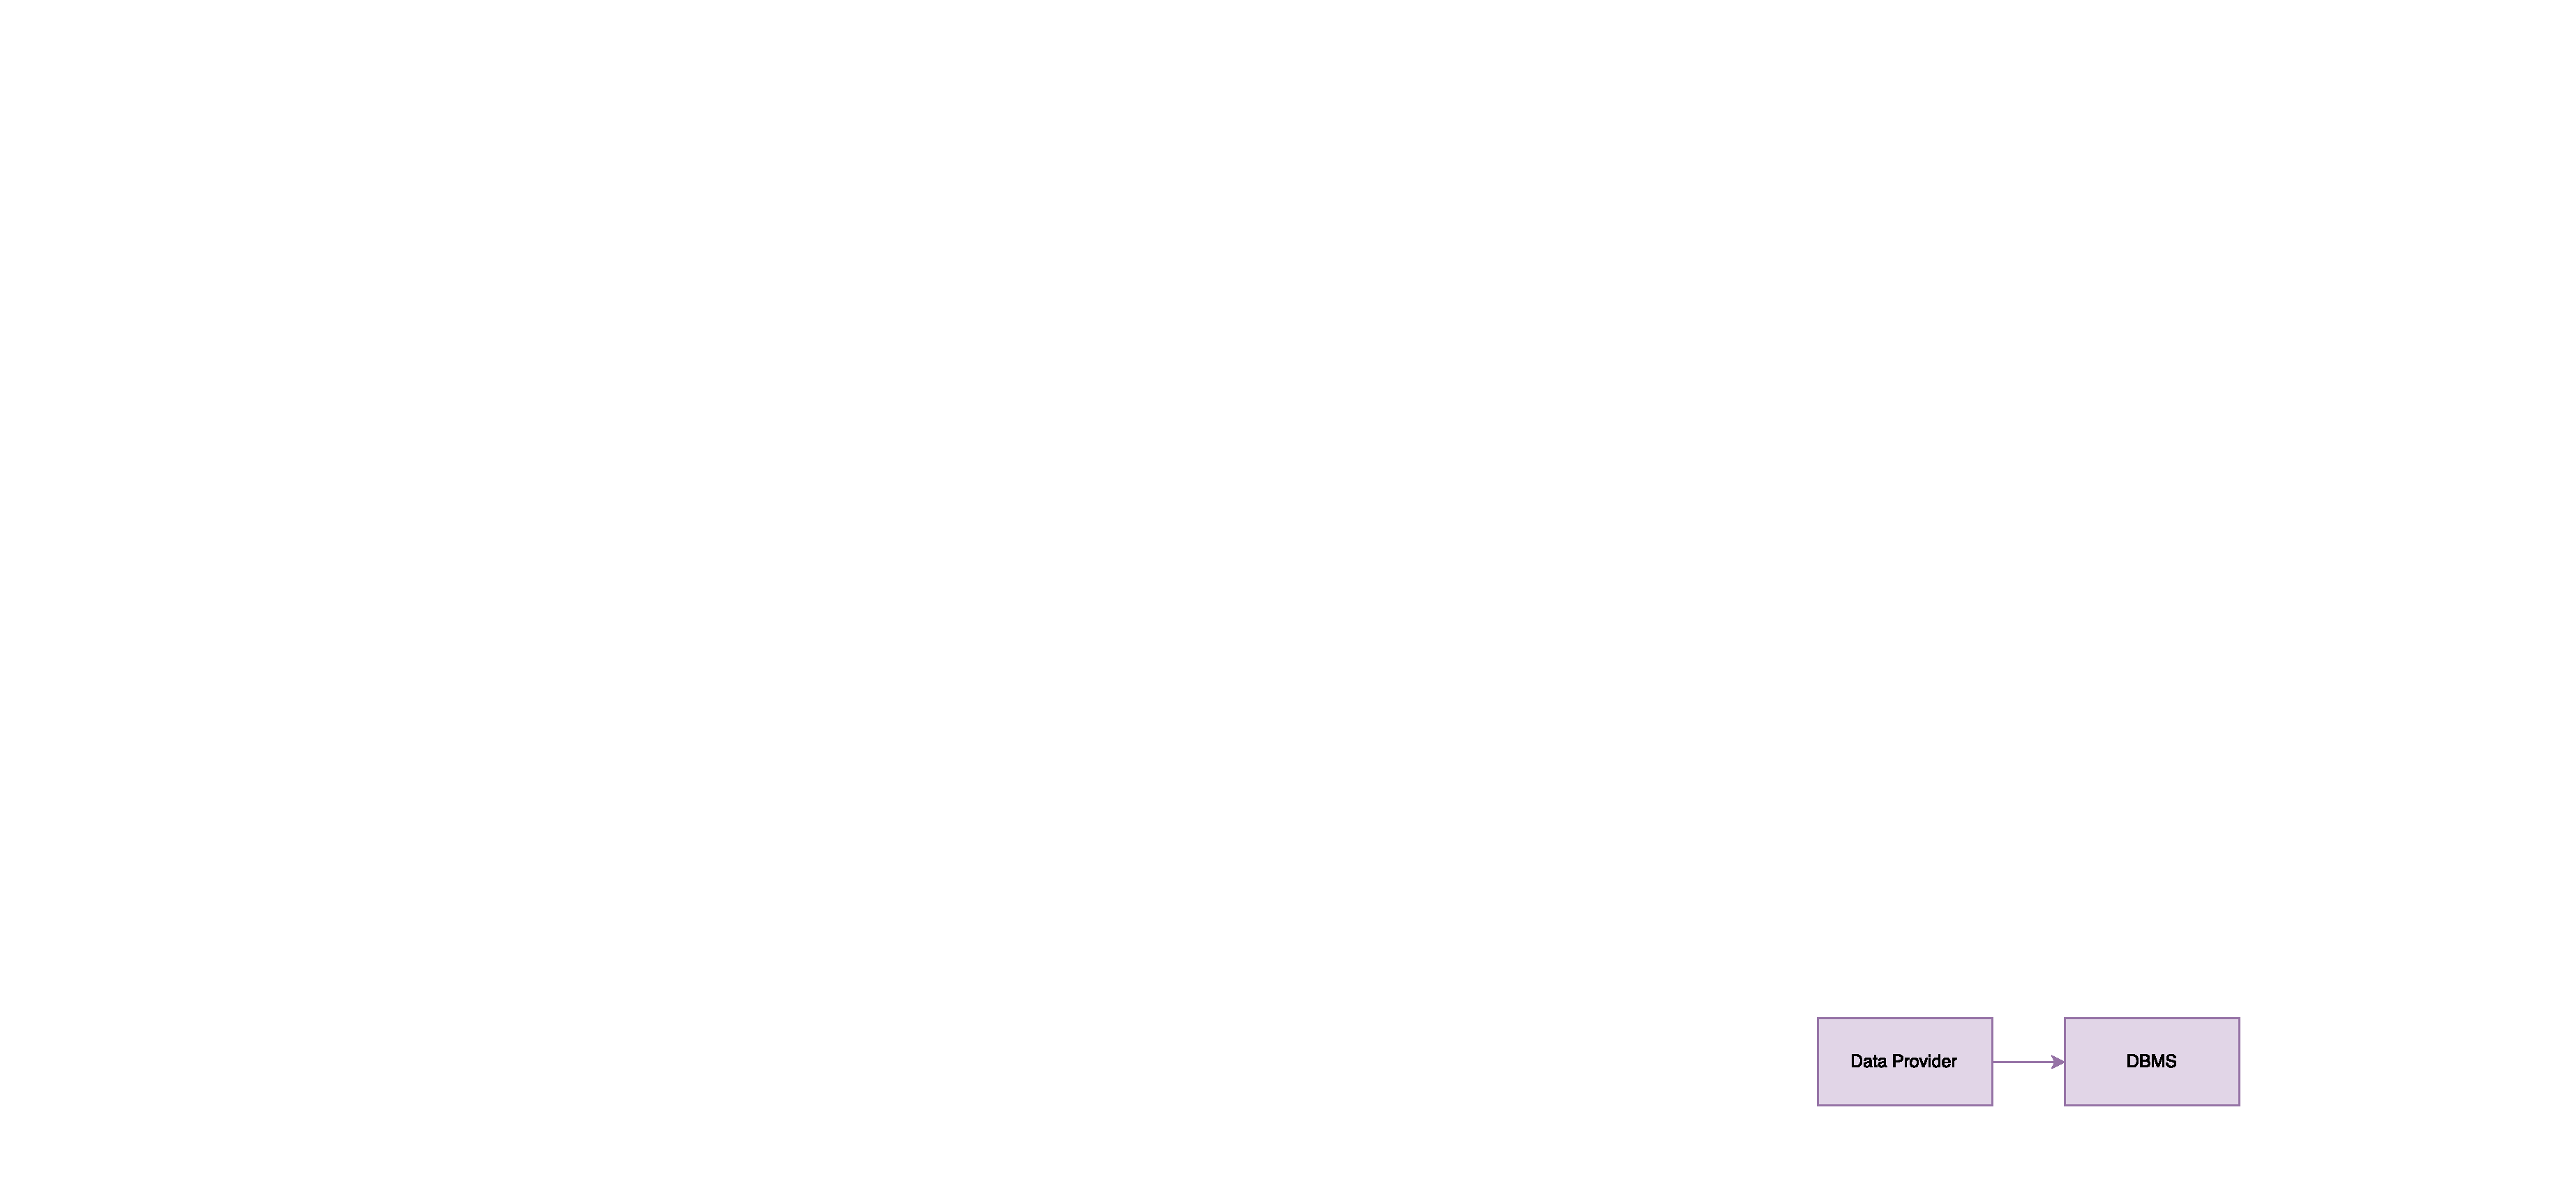
\includegraphics[width=0.6\linewidth]{img/Integration1}
			\caption{
				\label{fig:dataProvider} 
				\emph{DataProvider integration}
			}
		\end{figure}

\paragraph{EventBroker and CarHandler} 
...
\paragraph{}
		
		\begin{figure}[h]
			\centering
			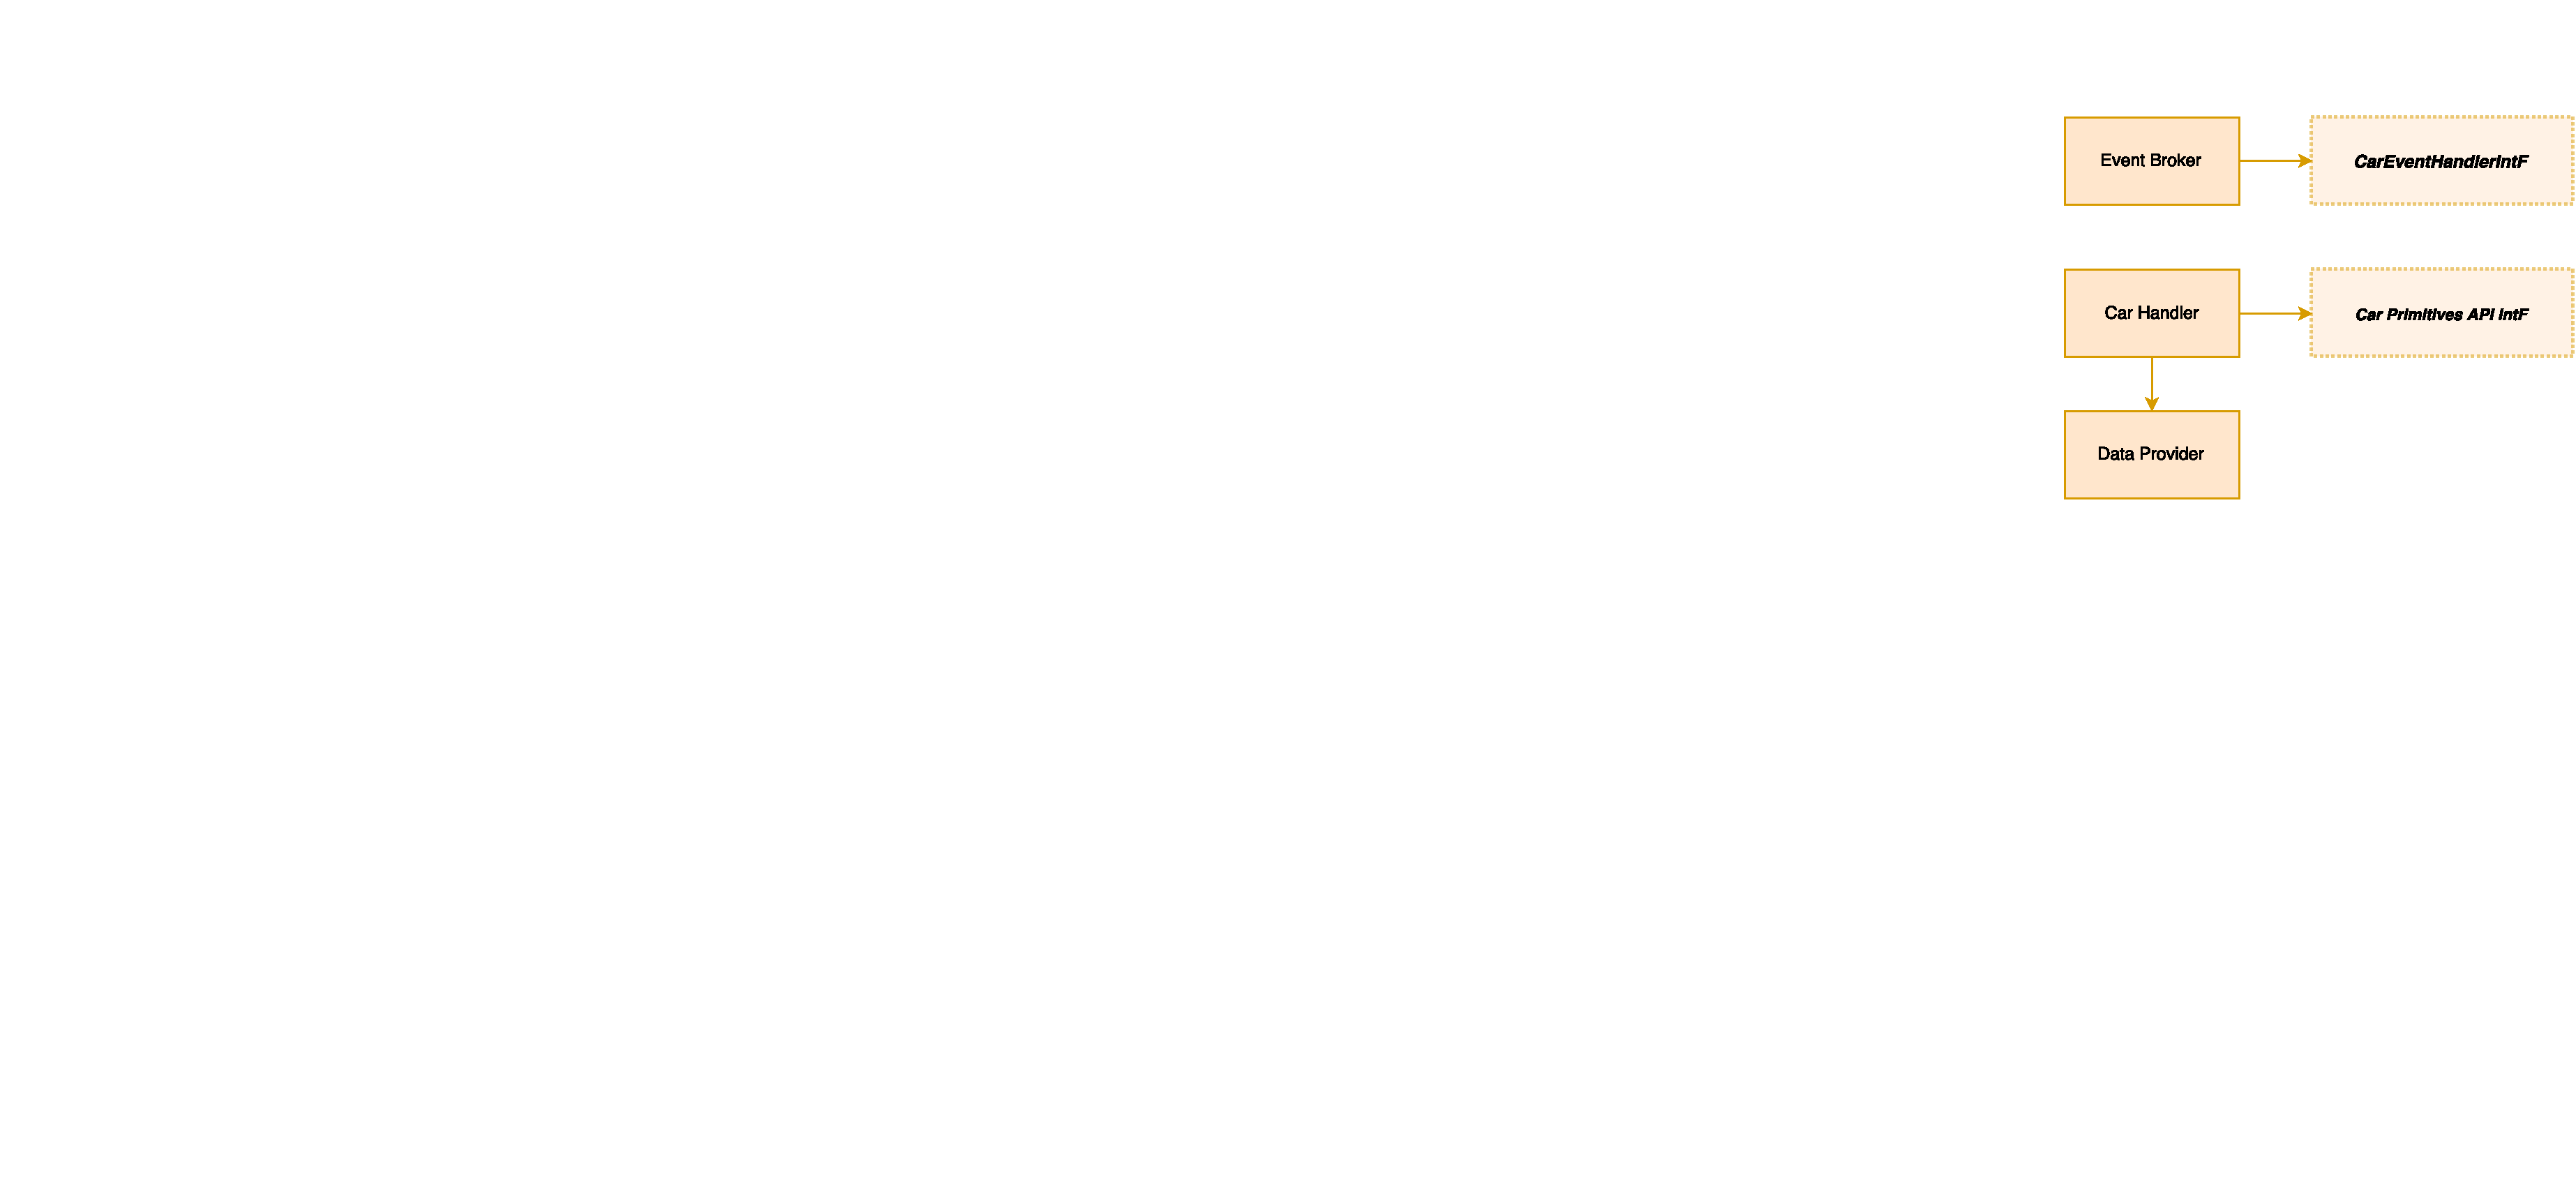
\includegraphics[width=0.6\linewidth]{img/Integration2a}
			\caption{
				\label{fig:eventBrokerCarHandler} 
				\emph{EventBroker and CarHandler integration}
			}
		\end{figure}

\paragraph{UserInformationManager and AccessManager} 
...
\paragraph{}
		
		\begin{figure}[h]
			\centering
			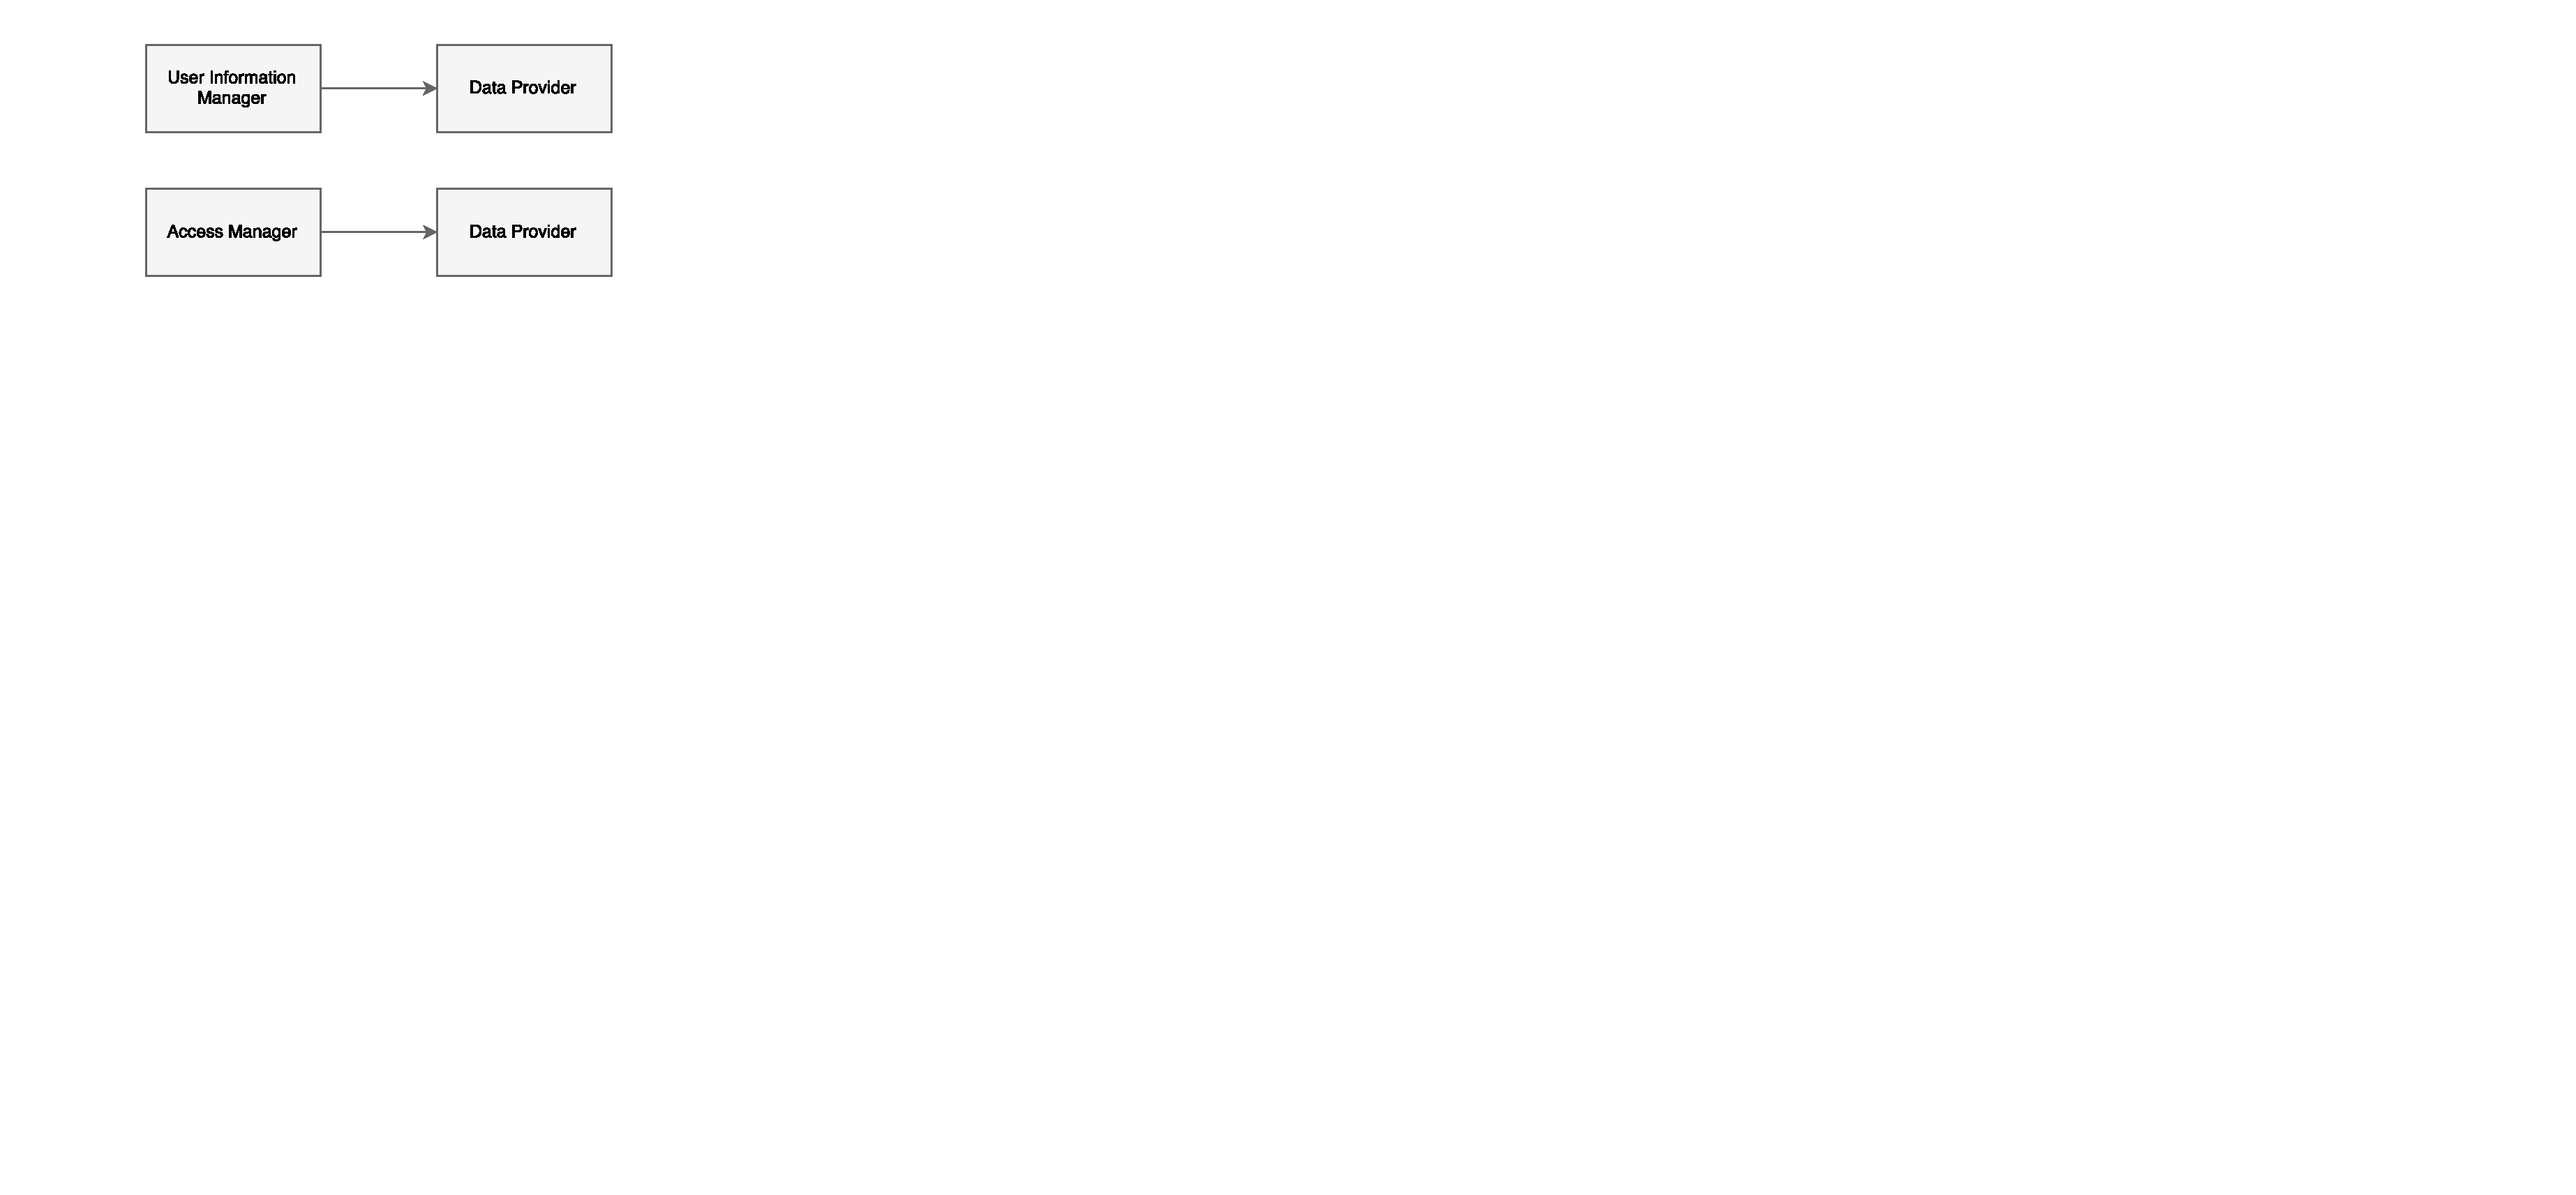
\includegraphics[width=0.6\linewidth]{img/Integration2b}
			\caption{
				\label{fig:userInfoAccessManager} 
				\emph{UserInformationManager and AccessManager integration}
			}
		\end{figure}
		
\paragraph{RentManager} 
...
\paragraph{}
		
		\begin{figure}[h]
			\centering
			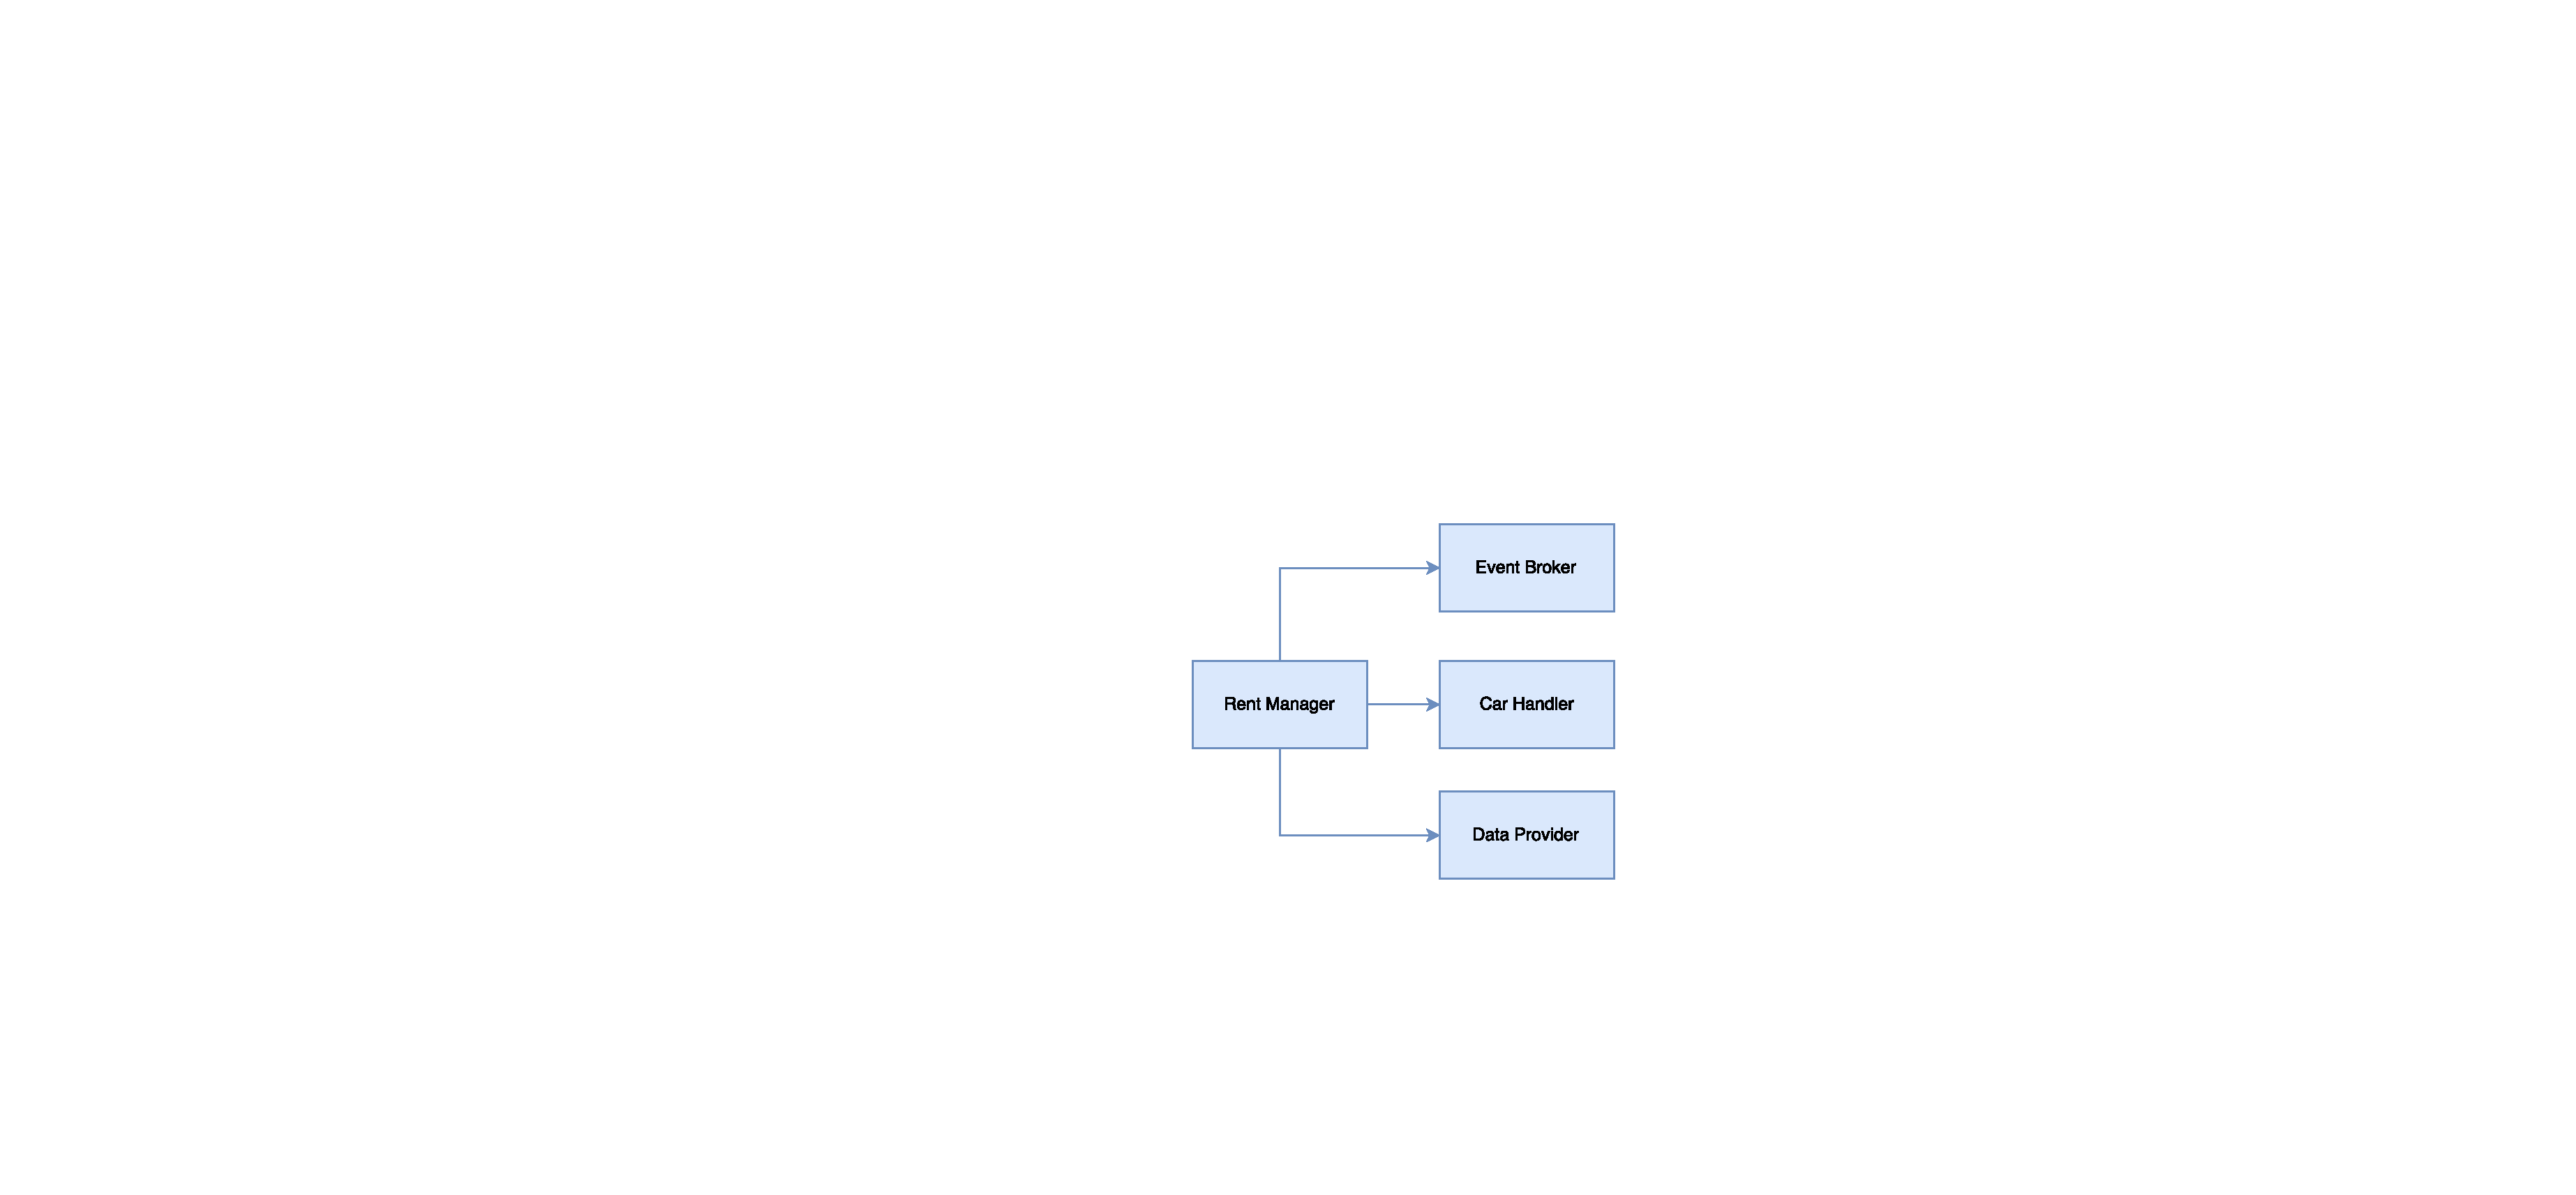
\includegraphics[width=0.8\linewidth]{img/Integration3a}
			\caption{
				\label{fig:rentManager} 
				\emph{RentManager integration}
			}
		\end{figure}

\paragraph{MaintenanceManager} 
...
\paragraph{}
		
		\begin{figure}[h]
			\centering
			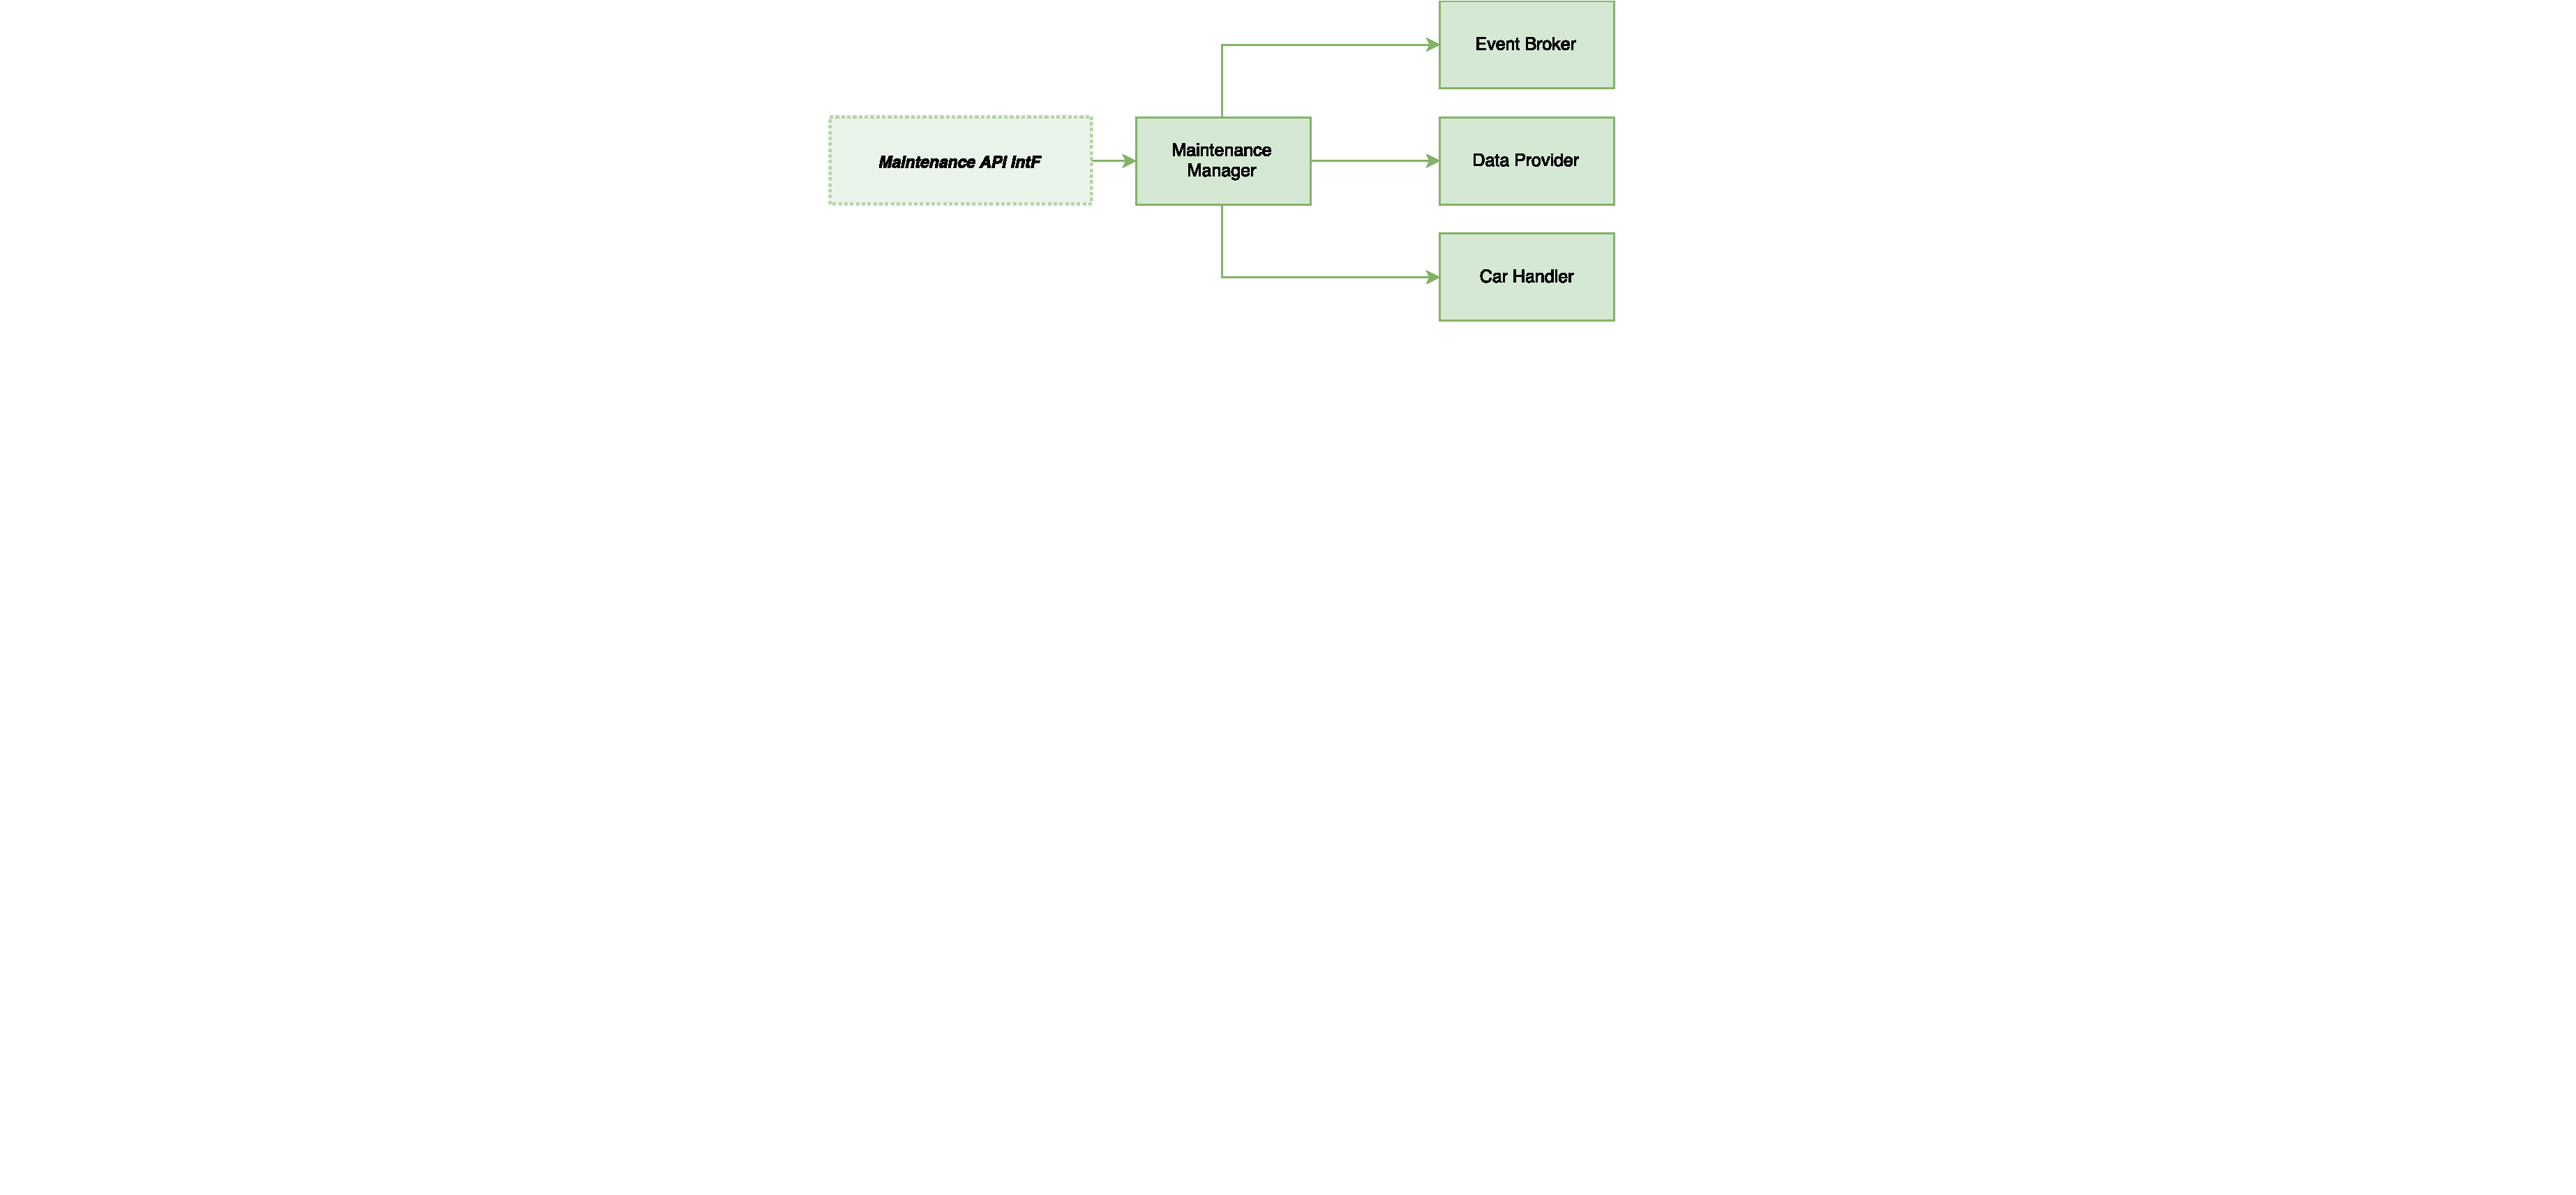
\includegraphics[width=0.8\linewidth]{img/Integration3b}
			\caption{
				\label{fig:maintenanceManager} 
				\emph{MaintenanceManager integration}
			}
		\end{figure}
		
\paragraph{CustomerCare Application and Server} 
...
\paragraph{}
		
		\begin{figure}[h]
			\centering
			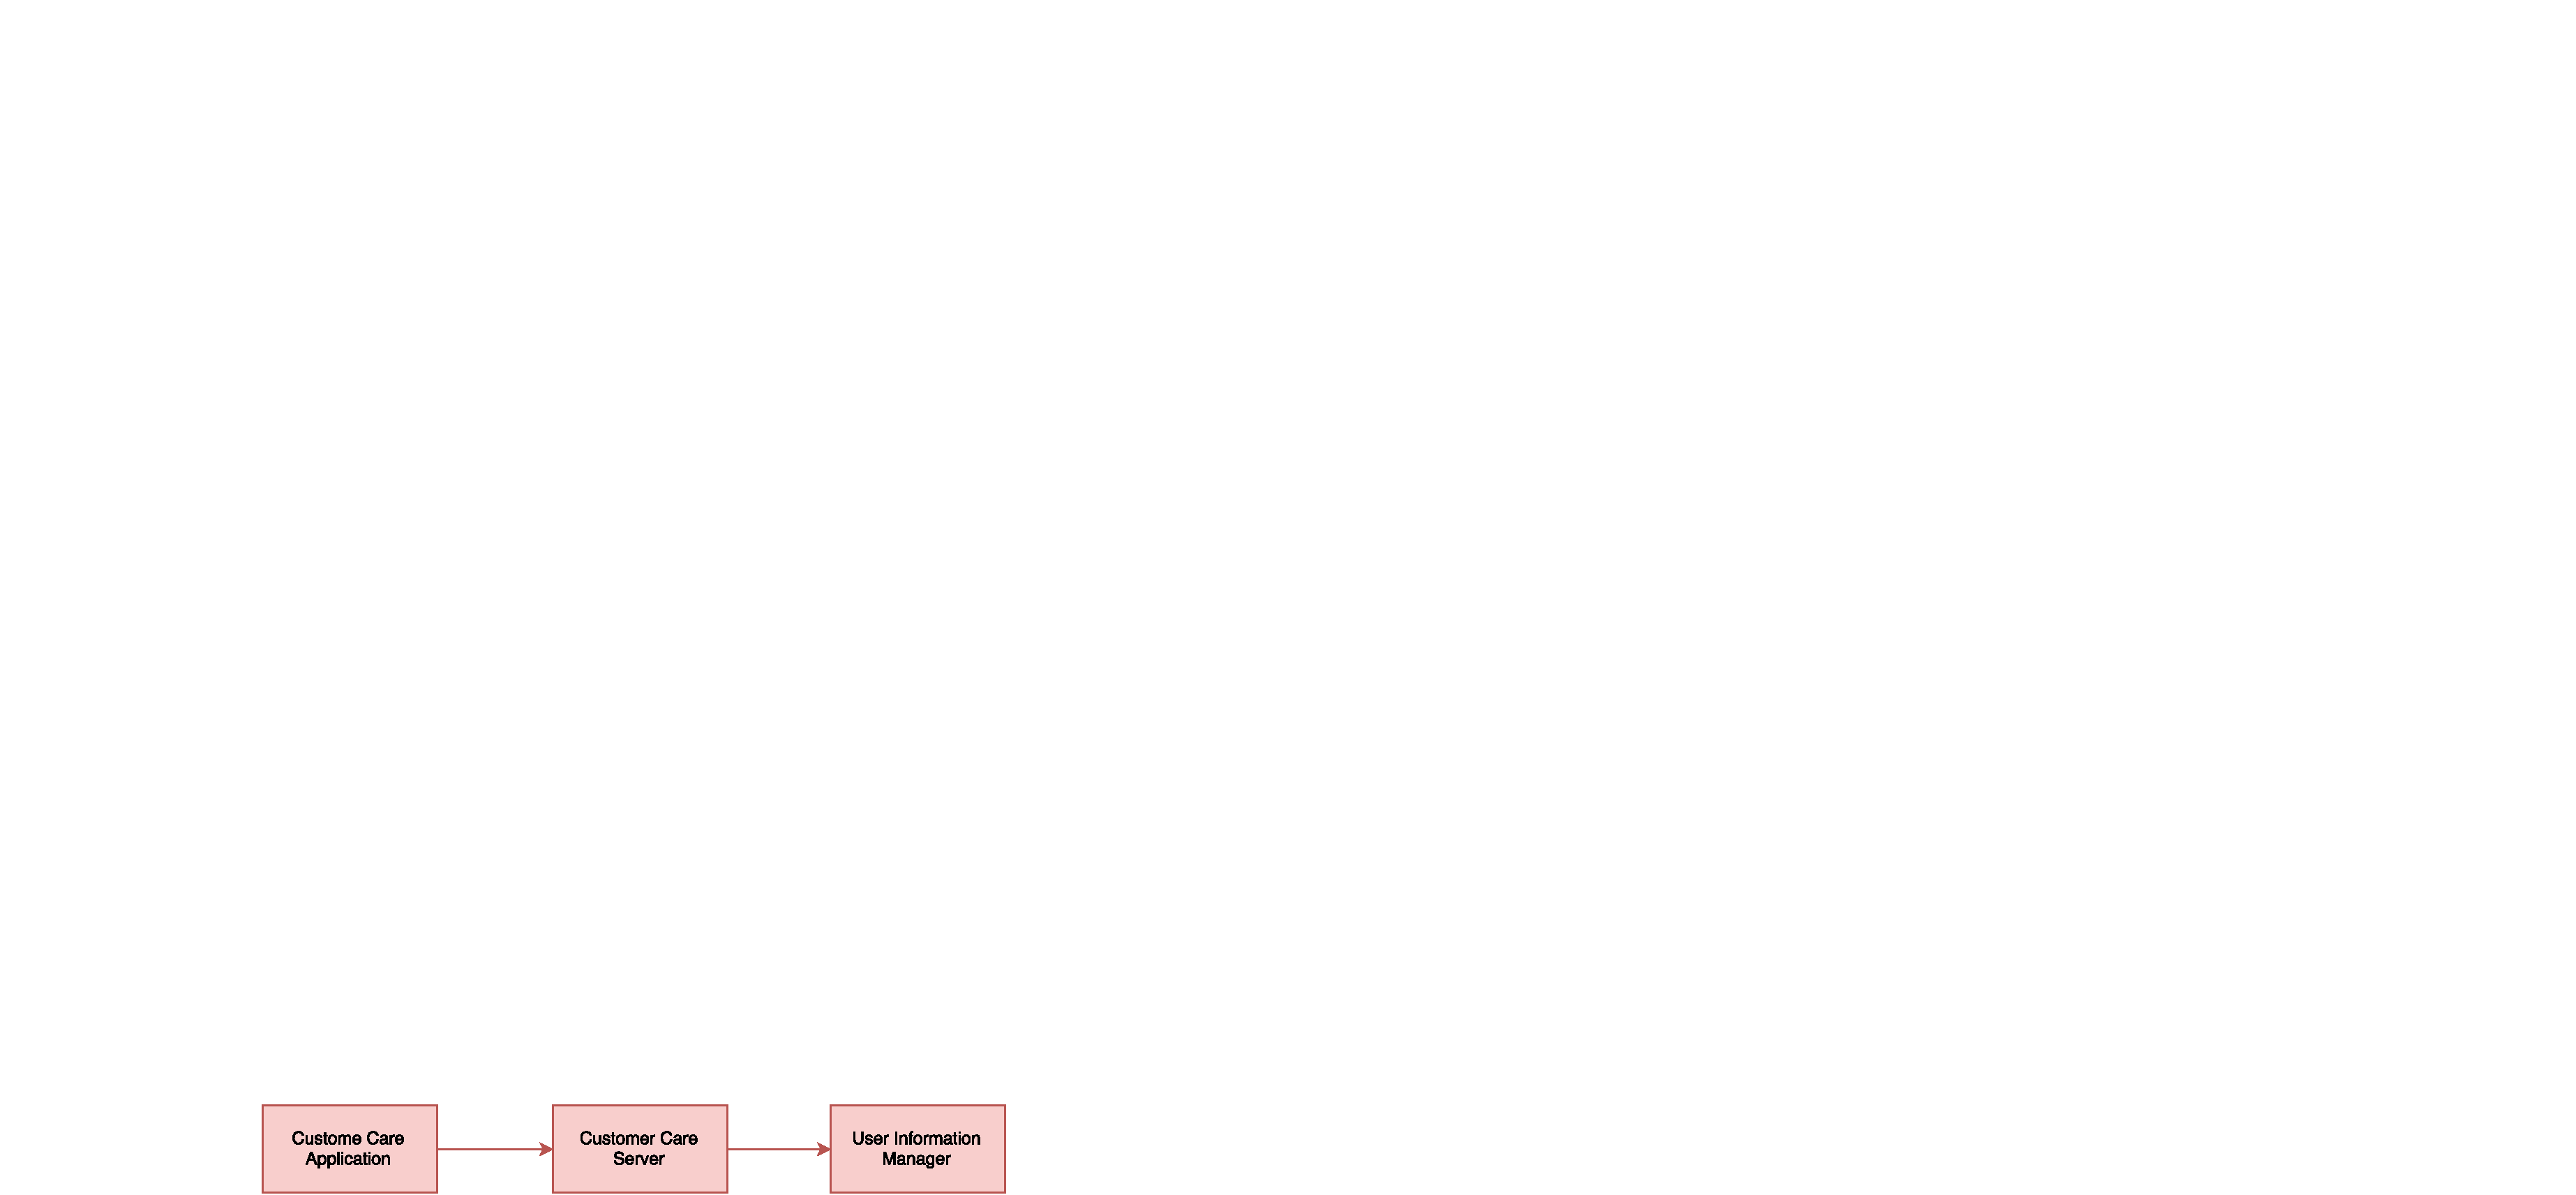
\includegraphics[width=0.8\linewidth]{img/Integration3c}
			\caption{
				\label{fig:ccAppServer} 
				\emph{CustomerCare Application and Server integration}
			}
		\end{figure}
		
\paragraph{User Application and Server} 
...
\paragraph{}
		
		\begin{figure}[h]
			\centering
			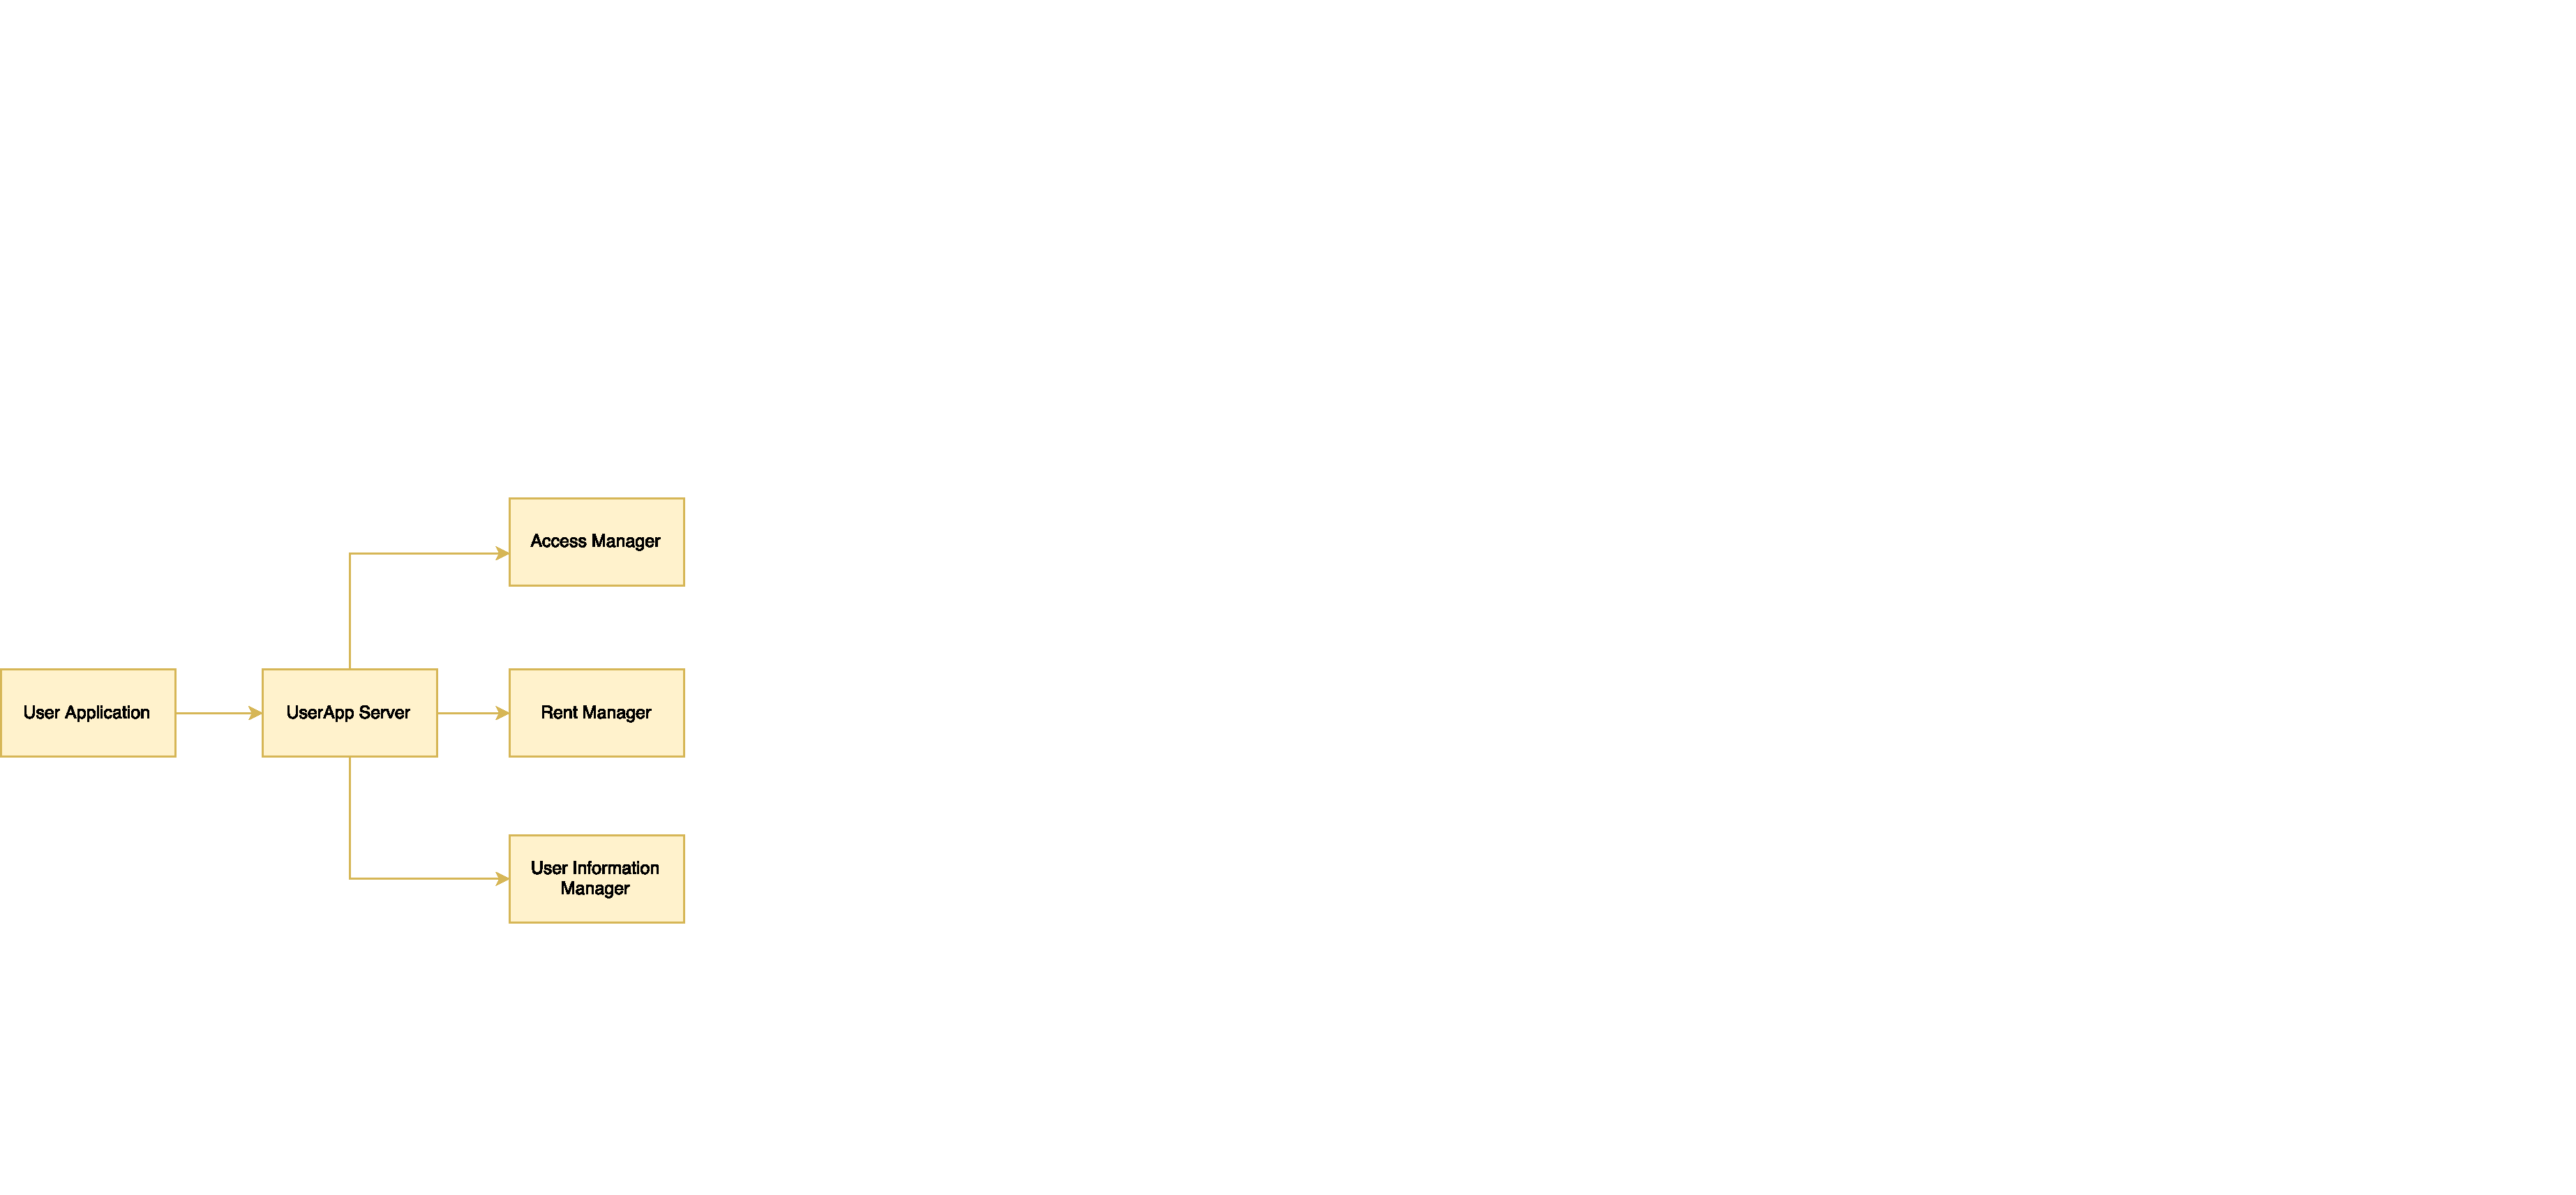
\includegraphics[width=0.8\linewidth]{img/Integration4}
			\caption{
				\label{fig:userAppServer} 
				\emph{User Application and Server integration}
			}
		\end{figure}

\clearpage 

\subsubsection{Subsystem Integration Sequence}

Unisco i sottosistemi del Maintenance (figura \ref{fig:maintenanceManager}), dello User (figura \ref{fig:userAppServer})  e del Customer Care (figura \ref{fig:ccAppServer}) nel sistema finale e testo tutto insieme. \todo{inglese}

	\begin{figure}[h]
			\centering
			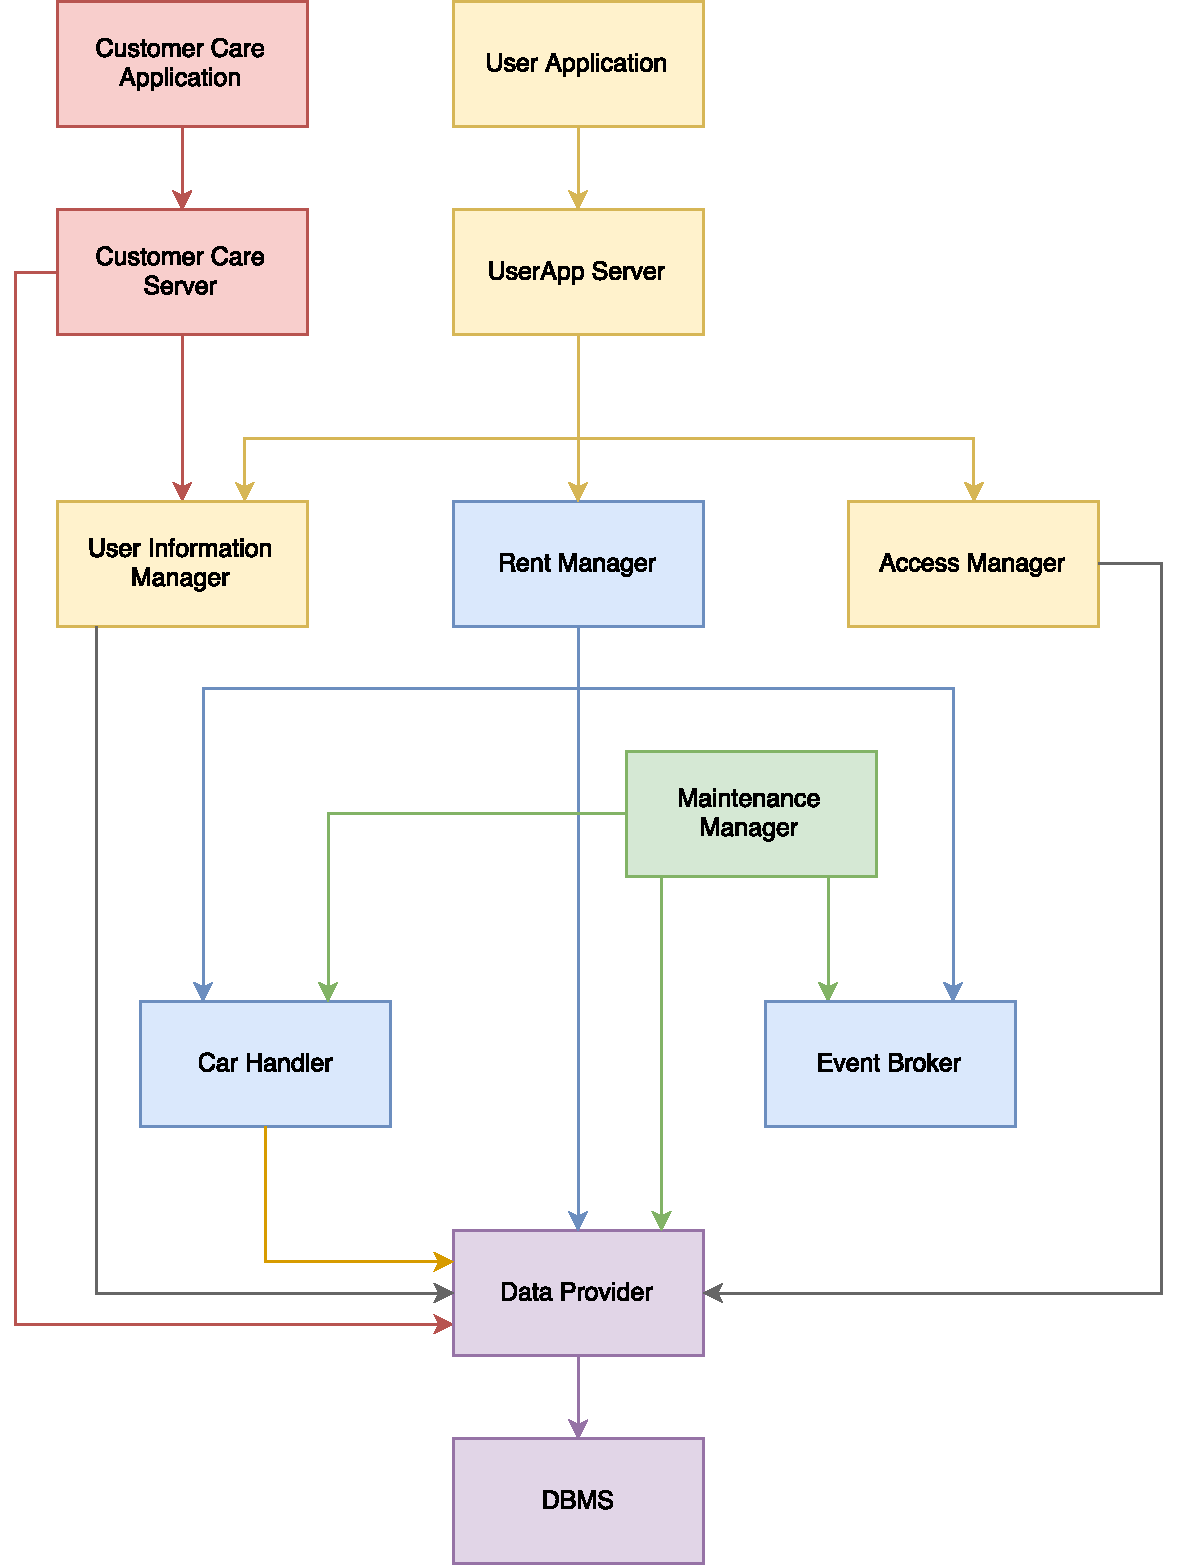
\includegraphics[width=0.8\linewidth]{img/subsystemIntegration}
			\caption{
				\label{fig:subsystemIntegration} 
				\emph{Subsystems Integration}
			}
		\end{figure}
